\documentclass{article}

\usepackage[a4paper]{geometry}
\usepackage[spanish]{babel}
\usepackage{xcolor}
\usepackage{placeins}

\usepackage{mathbbol}
\usepackage{amsmath}
\usepackage{amsfonts}
\usepackage{hyperref}
\usepackage{graphicx}
\usepackage{subcaption}

\usepackage{algorithm}
\usepackage{algpseudocode}

% Cambiar 'Cuadro' -> 'Tabla'
\addto\captionsspanish{
    \renewcommand{\tablename}{Tabla}
}

\begin{document}

\begin{center}
    {\Large Aprendizaje Automático para Datos en Grafos} \\
    {\LARGE \textbf{Laboratorio 4}} \\
    \vspace{2em}
    \begin{minipage}{0.45\textwidth}
        \centering
        Graciana Castro \\
        4.808.848-2 \\
        gcastro@fing.edu.uy
    \end{minipage}
    \hfill
    \begin{minipage}{0.45\textwidth}
        \centering
        Julian O'Flaherty \\
        6.285.986-9 \\
        julian.o.flaherty@fing.edu.uy
    \end{minipage}
\end{center}


\section{Introducción}

\section{Inferencia de topología en datos sintéticos}

\subsection{Generación del grafo sintético}

Para generar un grafo sintético, utilizaremos el siguiente algoritmo:
\begin{enumerate}
    \item Sorteamos $N$ puntos de forma uniforme en el cuadrado $[0,1] \times [0,1]$. Esos serán los vértices de nuestro grafo.
    \item Para cada par de puntos $i$ y $j$ que sorteamos antes, tomamos como peso de la arista
    \begin{equation*}
        w_{ij} = \begin{cases}
            0 & \text{si } i=j \\
            e^{-\frac{d(i,j)}{2\sigma^2}} & \text{si } i \neq j
        \end{cases}
    \end{equation*}
    donde $d(i,j)$ es la distancia euclidea en $\mathbb{R}^2$ y $\sigma$ es un parámetro fijo.
    \item Descartamos las aristas cuyo peso $w_{ij}$ sea menor que un número fijo $r>0$.
\end{enumerate}
En la figura~\ref{fig:grafo_sintetico} se muestra un grafo sintético generado con el algoritmo anterior para $N=50$, $\sigma=0.5$ y $r=0.6$.

\begin{figure}[htb]
    \centering
    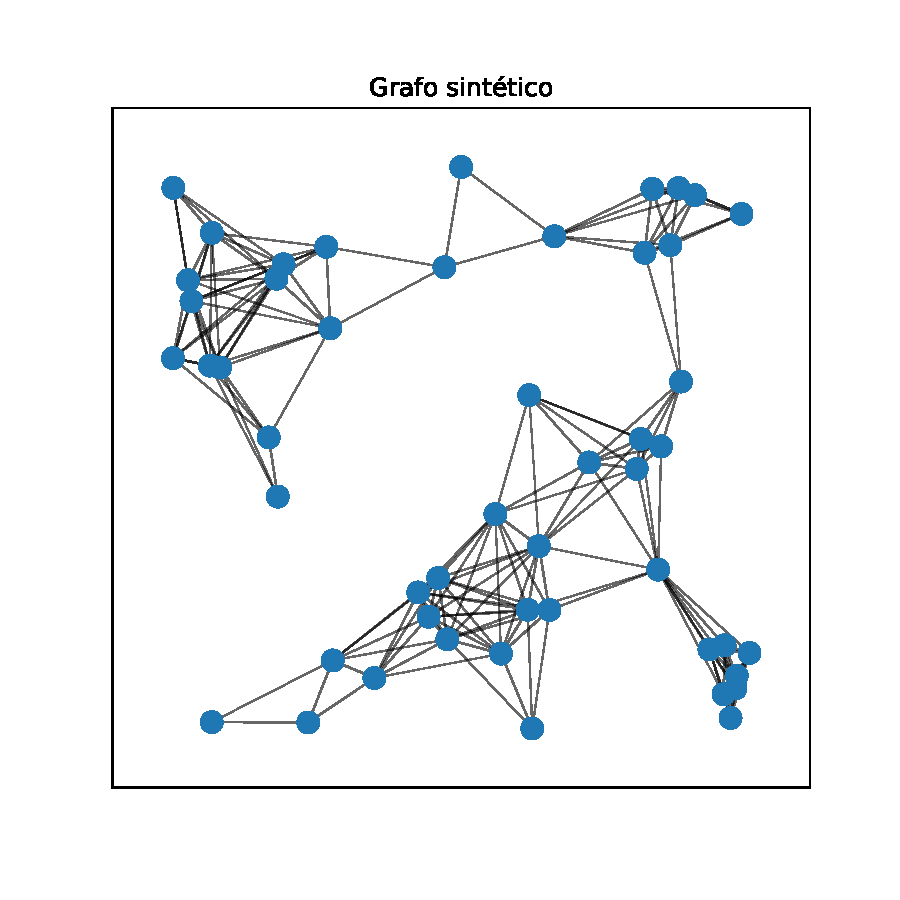
\includegraphics[width=0.5\textwidth]{imagenes/grafo_sintetico.pdf}
    \caption{Grafo sintético generado con $N=50$, $\sigma=0.5$ y $r=0.6$.}
    \label{fig:grafo_sintetico}
\end{figure}

A cada nodo del grafo sintetico, le asignaremos una señal $x_i \sim \mathcal{N}(0, \mathbf{L}^\dagger)$, donde $\mathbf{L}^\dagger$ es la pseudoinversa de la matriz laplaciana $\mathbf{L}$ del grafo. En la figura~\ref{fig:signals_X_pseudoinverse} se muestra un \textit{sample} de señales
donde cada columna $j$ es la señal asociada al nodo $j$ del grafo. La cantidad de filas, o el tamaño de la muestra, es el parámetro $n_{\text{samples}}$ del algoritmo, por lo que si $n_{\text{samples}}$ es menor que $N$, la matriz de covarianza empírica no es invertible.

\begin{figure}[htb]
    \centering
    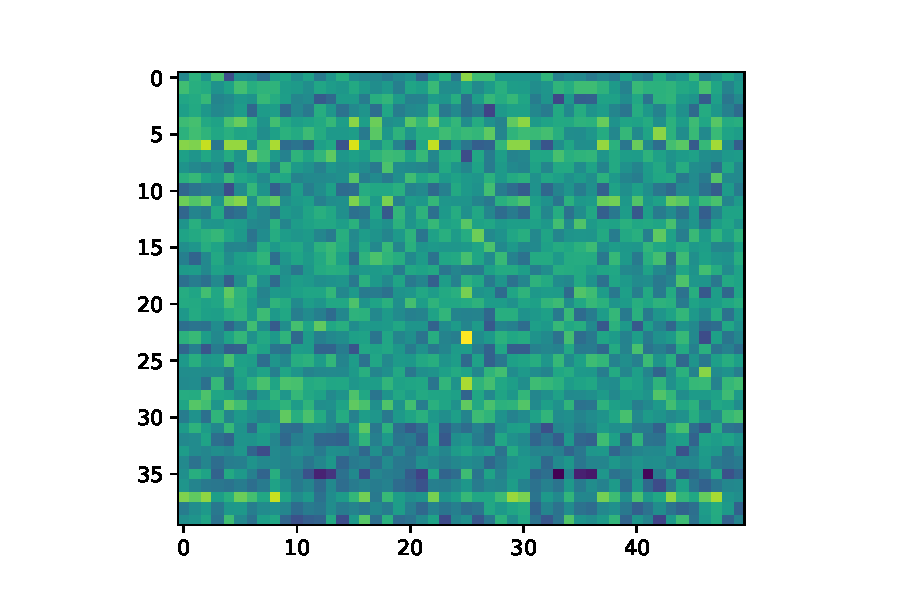
\includegraphics[width=0.6\textwidth]{imagenes/signals_X_pseudoinverse.pdf}
    \caption{Sample de señales asignadas a los nodos del grafo sintético.}
    \label{fig:signals_X_pseudoinverse}
\end{figure}

\subsection{Estimación de estructura con Graphical Lasso}

Estimaremos la estructura del grafo a partir de la matriz de datos utilizando el método \textit{Graphical Lasso}. Este método busca al estimador 
de máxima verosimilitud de la matriz de precisión $\boldsymbol{\Theta}$ que cumple:
\begin{equation}
\hat{\boldsymbol{\Theta}} = \arg \max_{\boldsymbol{\Theta} \succeq 0} \left\{ \log \det \boldsymbol{\Theta} - \text{trace}(\hat{\boldsymbol{\Sigma}} \boldsymbol{\Theta}) - \lambda \|\boldsymbol{\Theta}\|_1 \right\}
\end{equation}
Una de las propiedades importantes del Graphical Lasso, es que cuando $\lambda =  2\sqrt{\frac{\log N}{P}}$,
\begin{equation*}
    \|\hat{\boldsymbol{\Theta}} - \boldsymbol{\Theta}_0\|_2 \leq \sqrt{\frac{d_{\max}^2 \log N}{P}} \quad \text{w.h.p.}
\end{equation*}

con el parámetro $\lambda$ siendo parámetro de regularización. 
\begin{figure}[htb]
    \centering
    \begin{subfigure}[t]{0.32\linewidth}
        \centering
        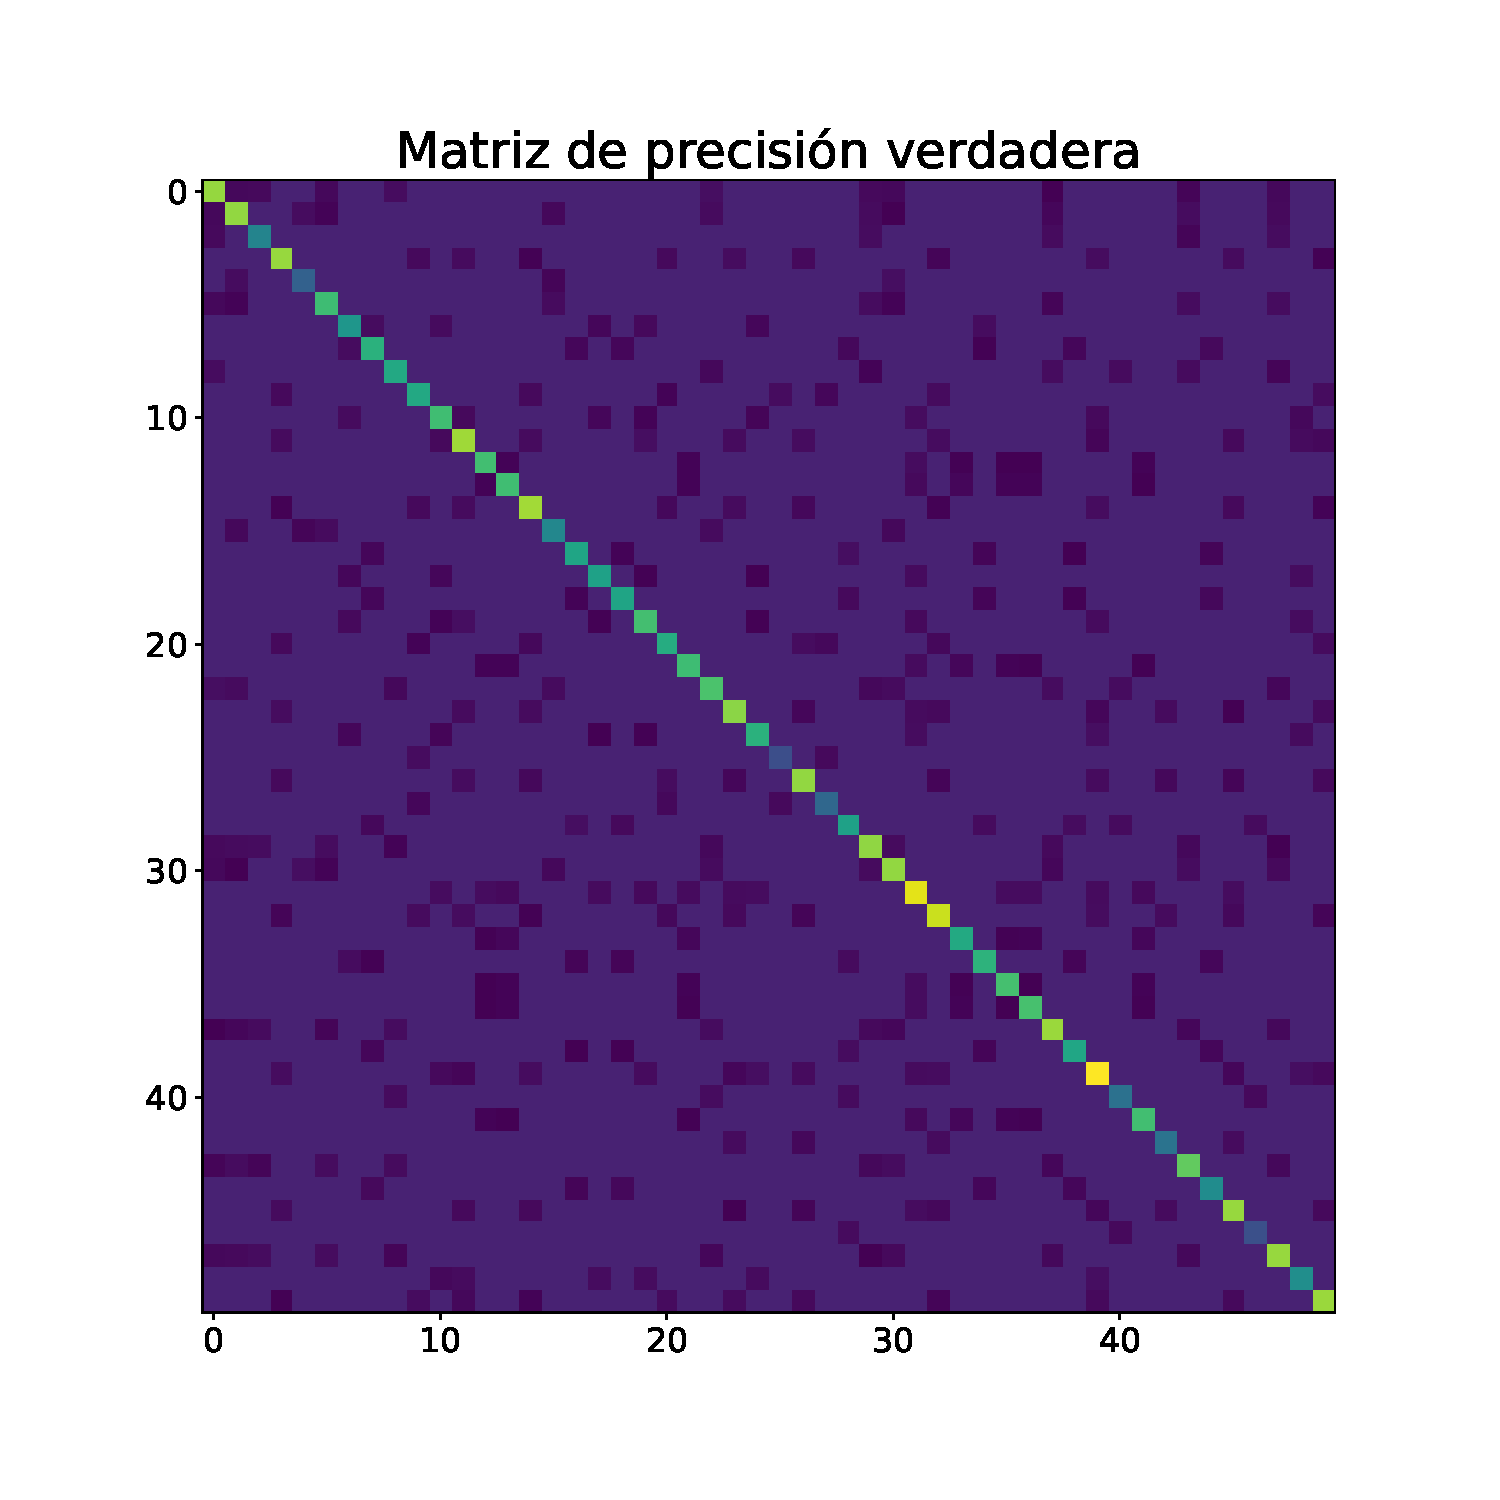
\includegraphics[width=\textwidth]{imagenes/graphical_lasso/true_precision_sample.pdf}
        \caption{Precisión verdadera}
        \label{fig:graphical_lasso_true_precision}
    \end{subfigure}\hfill
    \begin{subfigure}[t]{0.32\linewidth}
        \centering
        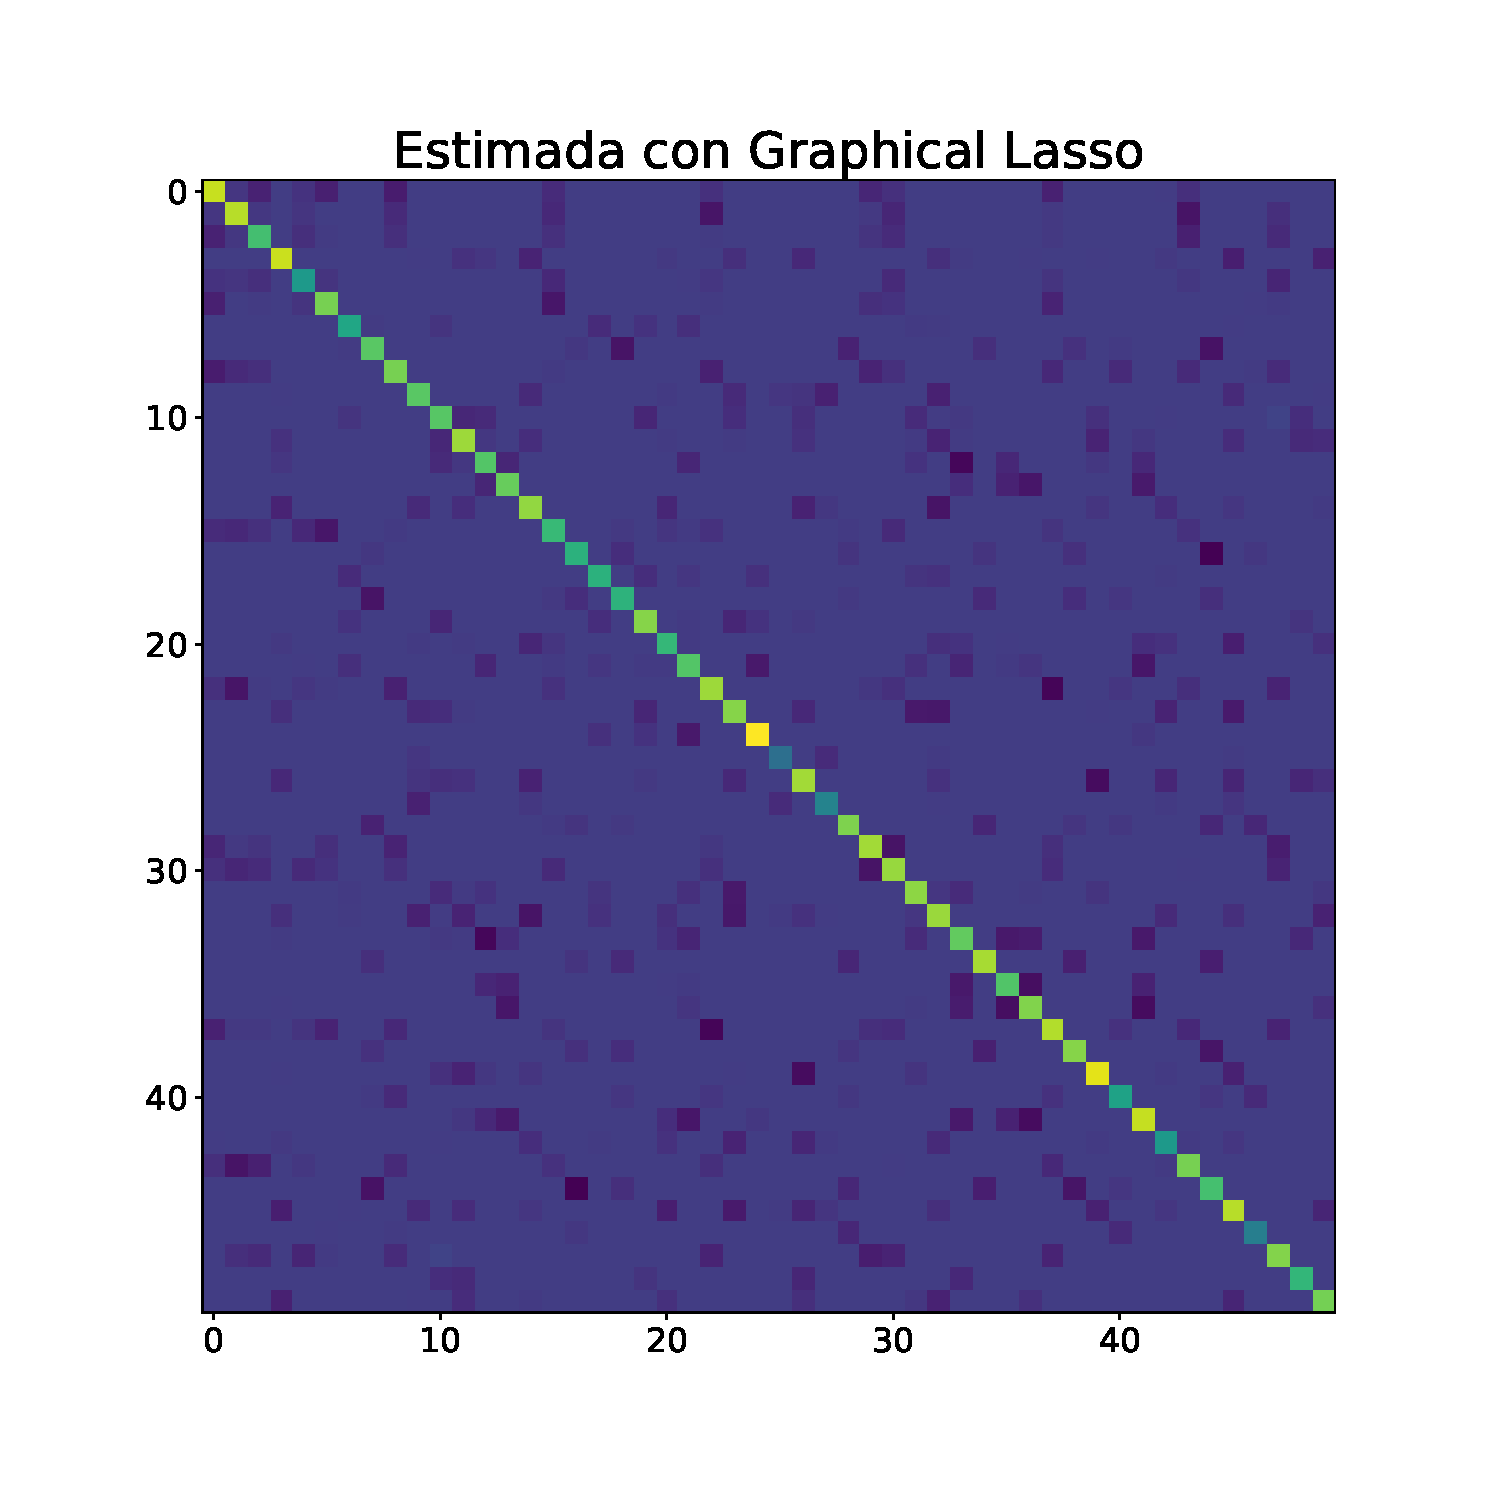
\includegraphics[width=\textwidth]{imagenes/graphical_lasso/graphical_sample.pdf}
        \caption{Estimación mediante Graphical Lasso}
    \end{subfigure}\hfill
    \begin{subfigure}[t]{0.32\linewidth}
        \centering
        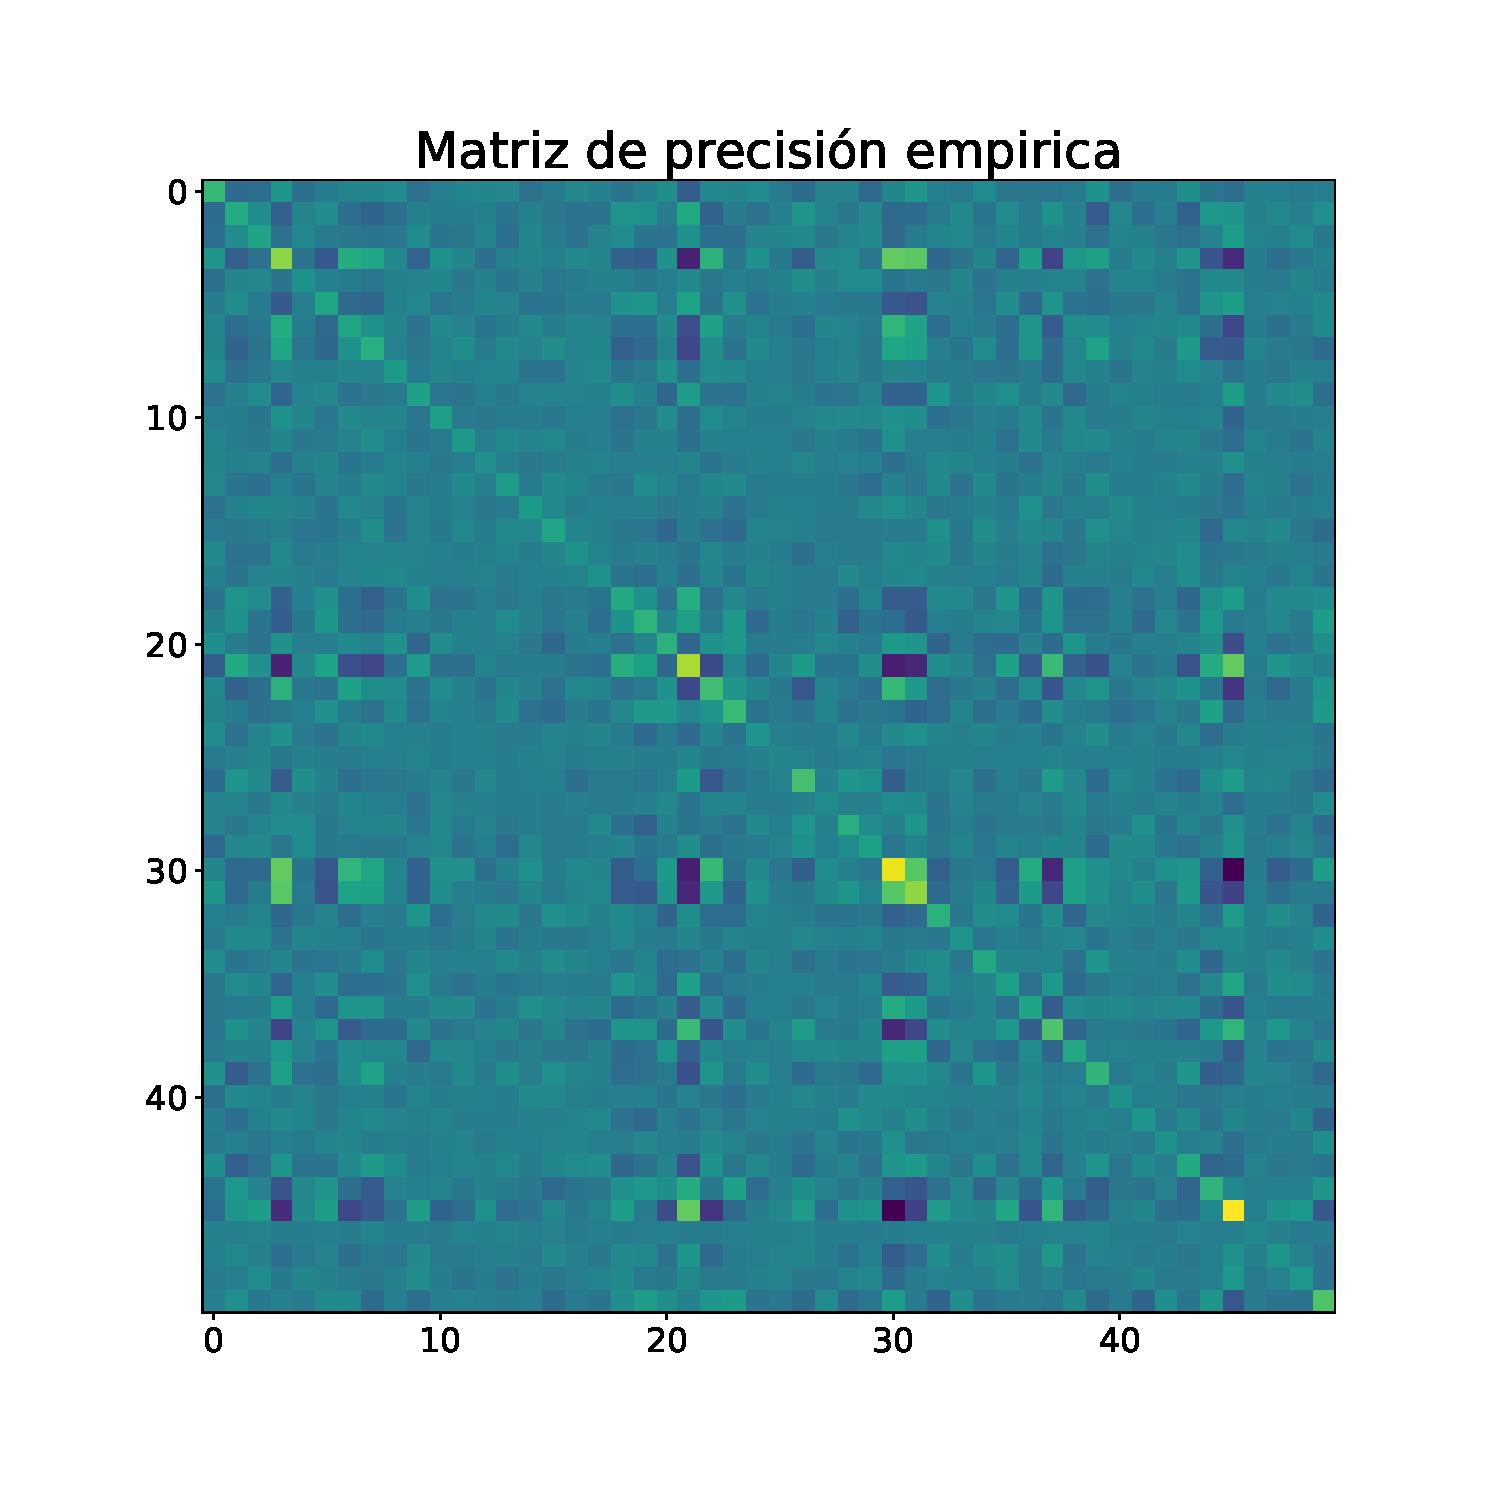
\includegraphics[width=\textwidth]{imagenes/graphical_lasso/estimated_sample.pdf}
        \caption{Estimación empírica \\ ($\Theta = \Sigma^{-1}$)}
    \end{subfigure}
    \caption{Comparación entre la matriz de precisión verdadera, la estimación mediante Graphical Lasso y la estimación obtenida con empíricamente ($\Theta = \Sigma^{-1}$), cuando $n_{\text{samples}}=40$ y $N=50$}
    \label{fig:graphical_lasso_triptych}
\end{figure}
En la figura~\ref{fig:graphical_lasso_triptych} se puede observar la estimación obtenida con \emph{Graphical Lasso} comparada con la estimación empírica cuando el número de samples utilizado $n_{\text{samples}}$ es menor que la cantidad de nodos $N$. En este caso, la estimación
empírica resulta mala, dado que la matriz de covarianza empírica no es invertible. El método de \emph{Graphical Lasso} obtiene un resultado muy similar a la matriz de precisión verdadera, donde el valor de $\lambda$ se calcula mediante validación cruzada. 

En la figura~\ref{fig:graphical_lasso_alpha_comparison} observamos el efecto del variar el valor de $\lambda$ sobre la matriz de precisión estimada. A medida que aumenta la regularización, la matriz va perdiendo ceros tendiendo a una matriz diagonal, lo cual es esperable
dado que el valor de $\lambda$ está asociado a la norma 1 de la matriz de precisión.
\begin{figure}[htb]
    \centering
    \begin{subfigure}[t]{0.32\linewidth}
        \centering
        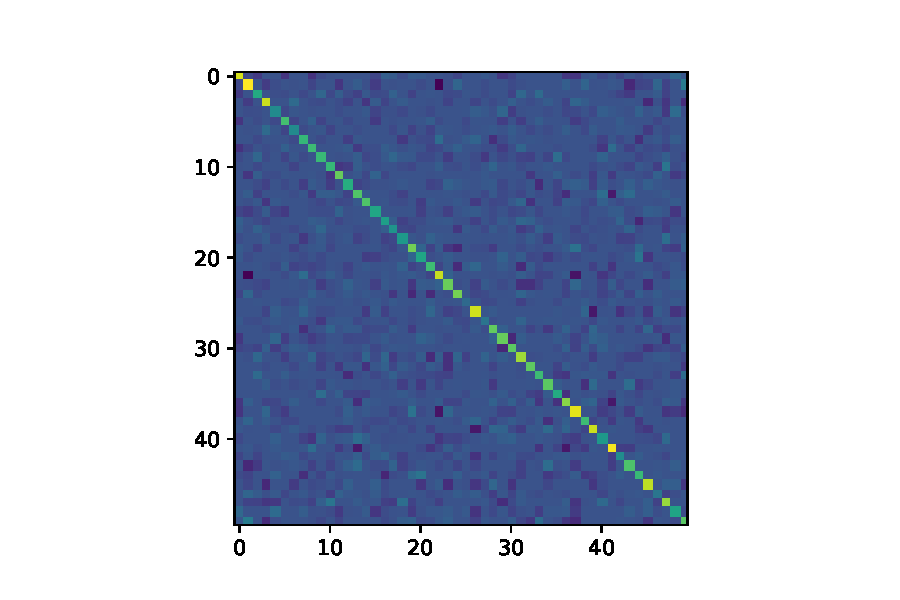
\includegraphics[width=\textwidth]{imagenes/graphical_lasso/graphical_lasso_alpha_0_01.pdf}
        \caption{$\lambda = 0.01$}
    \end{subfigure}\hfill
    \begin{subfigure}[t]{0.32\linewidth}
        \centering
        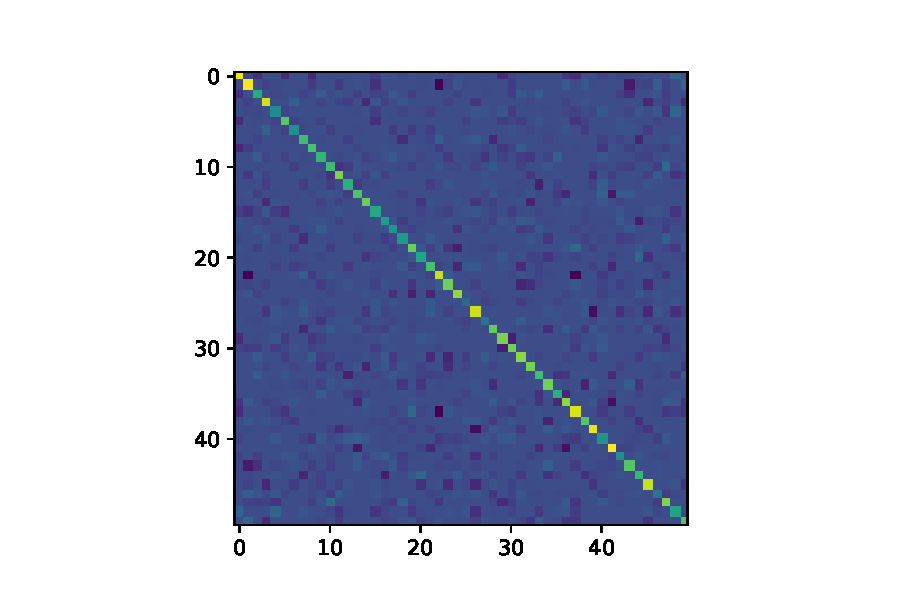
\includegraphics[width=\textwidth]{imagenes/graphical_lasso/graphical_lasso_alpha_0_02.pdf}
        \caption{$\lambda = 0.02$}
    \end{subfigure}\hfill
    \begin{subfigure}[t]{0.32\linewidth}
        \centering
        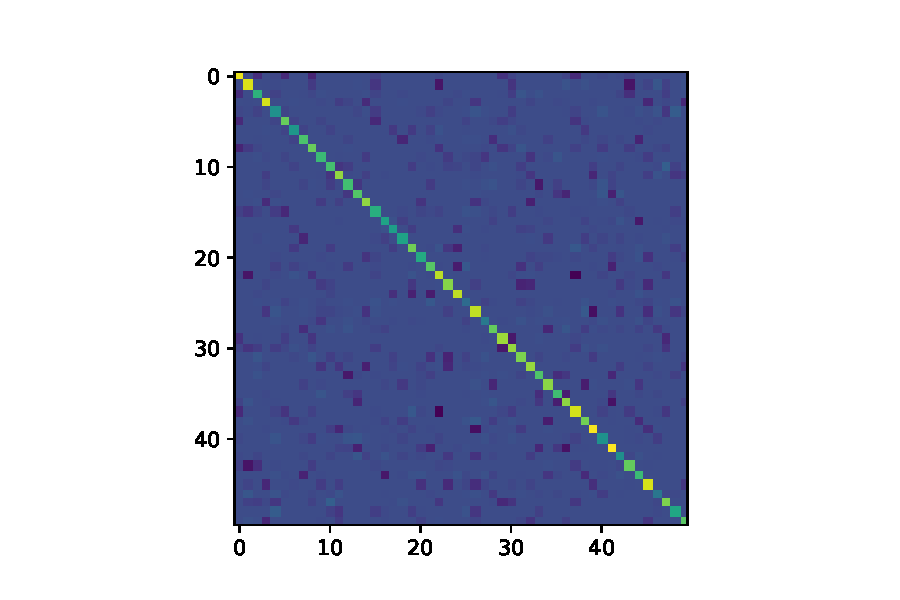
\includegraphics[width=\textwidth]{imagenes/graphical_lasso/graphical_lasso_alpha_0_05.pdf}
        \caption{$\lambda = 0.05$}
    \end{subfigure}
    \begin{subfigure}[t]{0.32\linewidth}
        \centering
        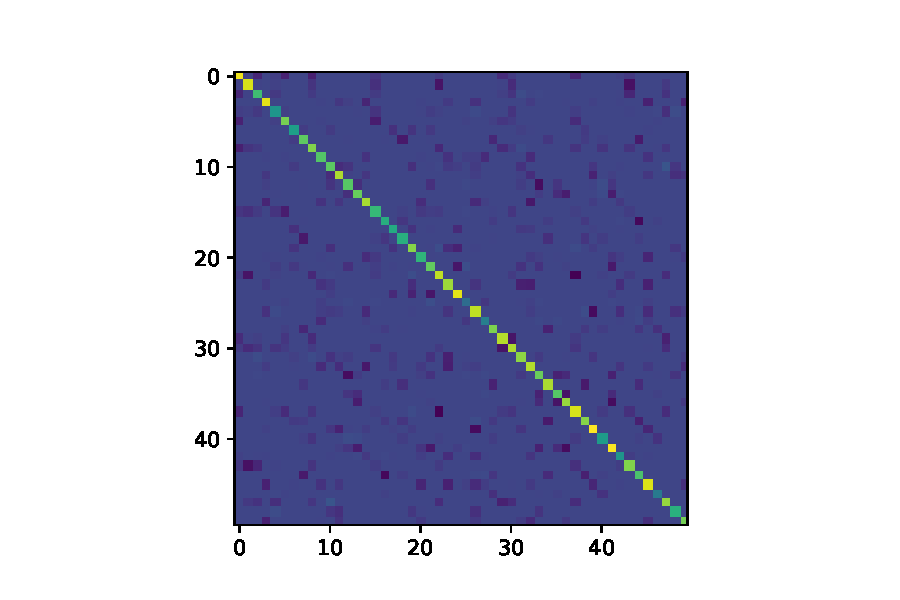
\includegraphics[width=\textwidth]{imagenes/graphical_lasso/graphical_lasso_alpha_0_1.pdf}
        \caption{$\lambda = 0.1$}
    \end{subfigure}
    \begin{subfigure}[t]{0.32\linewidth}
        \centering
        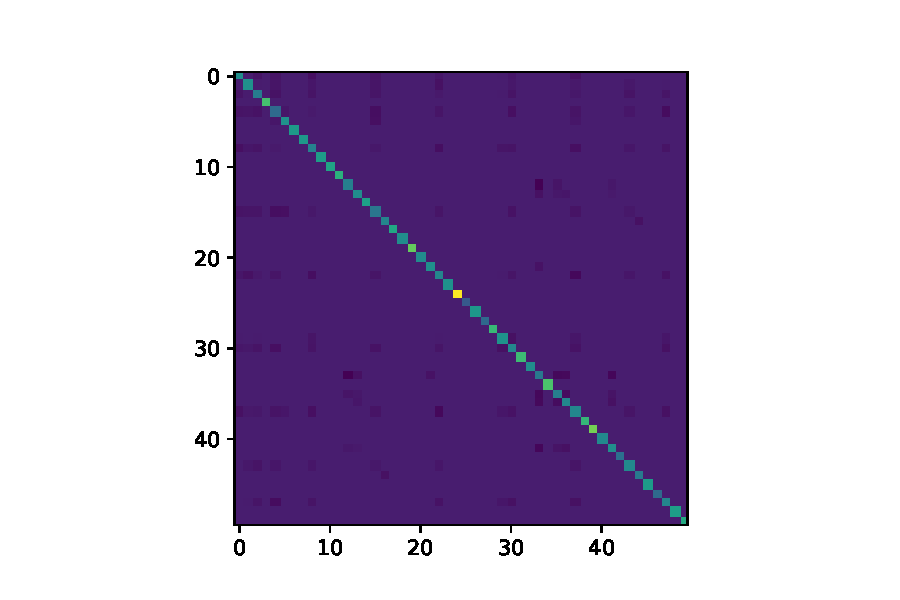
\includegraphics[width=\textwidth]{imagenes/graphical_lasso/graphical_lasso_alpha_0_5.pdf}
        \caption{$\lambda = 0.5$}
    \end{subfigure}
    \begin{subfigure}[t]{0.32\linewidth}
        \centering
        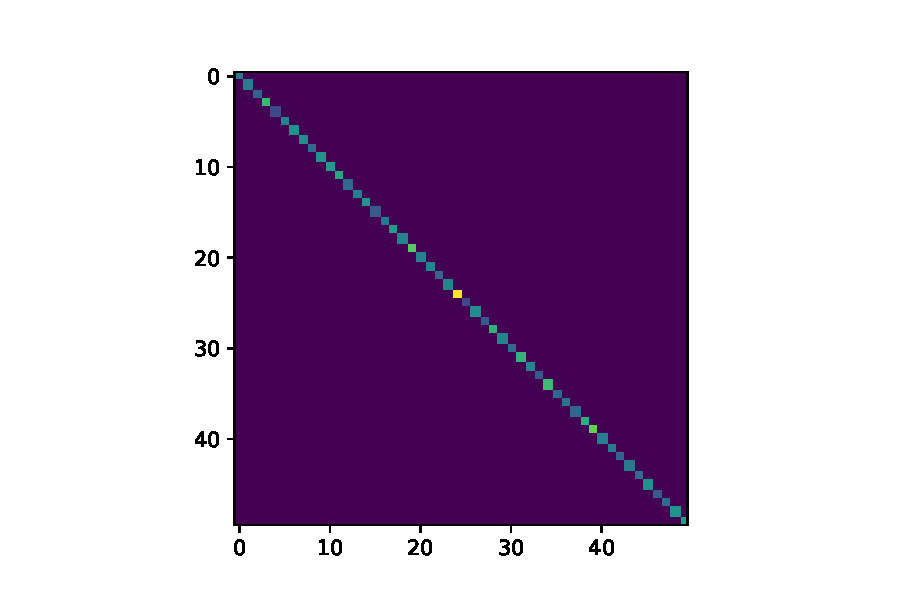
\includegraphics[width=\textwidth]{imagenes/graphical_lasso/graphical_lasso_alpha_1.pdf}
        \caption{$\lambda = 1$}
    \end{subfigure}
    \caption{Estimación mediante Graphical Lasso para distintos valores de $\lambda$. La matriz de precisión verdadera se muestra en la figura~\ref{fig:graphical_lasso_true_precision}. No se muestran valores menores a $0.01$ porque hay poca diferencia notable, y a partir de $0.005$ el sistema queda mal condicionado y no puede ser resuelto.
}
    \label{fig:graphical_lasso_alpha_comparison}
\end{figure}

\subsection{Estimación de estructura con Meinshausen y Bühlmann}

\subsection{Estimación de estructura con Meinshausen y Bühlmann}

El método de Meinshausen y Bühlmann propone una alternativa eficiente para la estimación de la estructura de grafos mediante selección de vecindarios con Lasso. Este método es particularmente útil en problemas de alta dimensionalidad donde $p \gg n$, ya que permite identificar los ceros estructurales en la matriz de precisión que representan restricciones de independencia condicional entre variables.

La idea central consiste en estimar el vecindario de cada nodo de forma individual mediante regresión. Para cada nodo $a$, se define su vecindario como el conjunto mínimo de variables que, al ser conocidas, hacen que $X_a$ sea condicionalmente independiente del resto. Esto se formula como un problema de regresión Lasso donde $X_a$ es la variable respuesta y las demás son predictoras:

\begin{equation}
    \hat{\theta}_{a,\lambda} = \operatorname*{argmin}_{\theta : \theta_a=0} \left(n^{-1}\|X_a - X\theta\|_2^2 + \lambda\|\theta\|_1\right)
\end{equation}

El vecindario estimado de $a$ se determina por los coeficientes no nulos de $\hat{\theta}_{a,\lambda}$. Una vez obtenidos todos los vecindarios, el conjunto de aristas del grafo se construye mediante la regla AND:

\begin{equation}
    \hat{E}_{\lambda, \wedge} = \{(a, b) : a \in \hat{n}e_{\lambda, b} \land b \in \hat{n}e_{\lambda, a}\}
\end{equation}

Una propiedad importante de este método es que mantiene consistencia incluso cuando $p \gg n$, siempre que el parámetro $\lambda$ se elija adecuadamente.

Para implementar este método, seguimos el siguiente algoritmo:
\begin{enumerate}
    \item Normalizamos la matriz de datos $\mathbf{X}$ por columnas.
    \item Inicializamos una matriz $\mathbf{B}$ de ceros de tamaño $p \times p$.
    \item Para cada nodo $j$ del grafo:
    \begin{enumerate}
        \item Extraemos la columna $j$ de $\mathbf{X}$ como variable objetivo $\mathbf{y}_j$.
        \item Utilizamos las demás columnas como matriz de predictores $\mathbf{X}_j$.
        \item Resolvemos el problema de regresión Lasso para obtener los coeficientes $\hat{\boldsymbol{\theta}}_j$.
        \item Insertamos los coeficientes en la fila $j$ de $\mathbf{B}$, colocando un cero en la posición $j$.
    \end{enumerate}
    \item Devolvemos la matriz $\mathbf{B}$ que contiene los coeficientes de regresión para cada nodo.
\end{enumerate}

En la figura \ref{fig: meinhausen} se observa que el método de Meinshausen y Bühlmann logra capturar la estructura principal de la matriz de coeficientes verdadera, identificando correctamente las conexiones más relevantes. Sin embargo, aparecen algunos falsos positivos y negativos, lo que refleja el compromiso entre detección y ruido inherente al uso de Lasso.

\begin{figure}[htb]
    \centering
    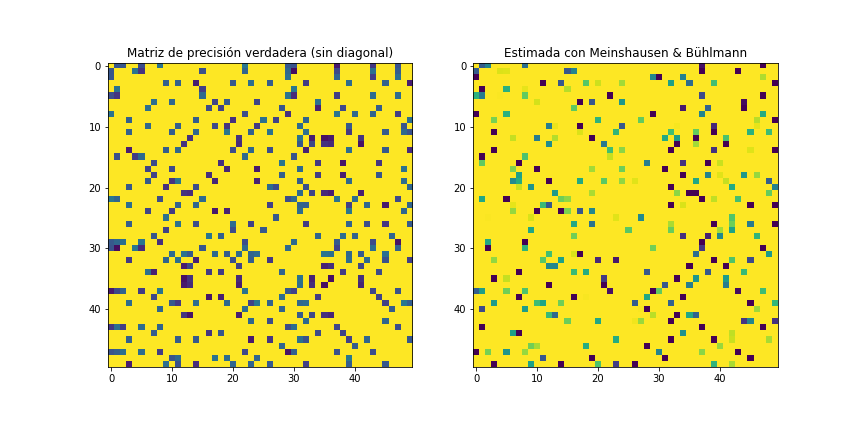
\includegraphics[width=0.6\textwidth]{imagenes/meinhausen/matriz_estimada.png}
    \caption{Comparación entre la matriz de coeficientes verdadera y la matriz de coeficientes estimada con el método de Meinshausen y Bühlmann.}
    \label{fig: meinhausen}
\end{figure}

\subsection{Estimación de estructura con Kalofolias}
El método propuesto por Kalofolias plantea aprender la estructura de un grafo a partir de señales que residen en sus nodos, asumiendo que estas señales cambian suavemente entre nodos conectados. La contribución clave consiste en reformular el problema tradicional de minimización del término de suavidad $\text{tr}(X^T L X)$ mostrando que es equivalente a una norma $\ell_1$ ponderada aplicada a la matriz de adyacencia $W$:

\begin{equation}
\text{tr}(X^T L X) = \frac{1}{2} \|W \circ Z\|_{1,1}
\end{equation}

donde $Z_{i,j} = \|x_i - x_j\|_2$ es la matriz de distancias por pares entre las señales. Esta equivalencia permite formular el problema de aprender el grafo como:

\begin{equation}
\min_{W \in \mathcal{W}_m} \|W \circ Z\|_{1,1} - \alpha \mathbf{1}^T \log(W \mathbf{1}) + \beta \|W\|_F^2
\end{equation}

El término logarítmico $-\alpha \mathbf{1}^T \log(W \mathbf{1})$ actúa sobre el vector de grados de los nodos, promoviendo la conectividad del grafo, mientras que el término $\beta \|W\|_F^2$ controla la dispersión de los pesos. Los parámetros $\alpha > 0$ y $\beta \geq 0$ permiten balancear estos objetivos.

En la figura \ref{fig:kalofolias_grid} se presentan los resultados obtenidos con diferentes combinaciones de $\alpha$ y $\beta$, comparados con la matriz verdadera. Se aprecia cómo estos parámetros influyen en la estructura del grafo aprendido, permitiendo ajustar el balance entre conectividad y dispersión de pesos según las características deseadas.

\begin{figure}[htb]
    \centering
    \begin{minipage}[t]{0.25\textwidth}
        \centering
        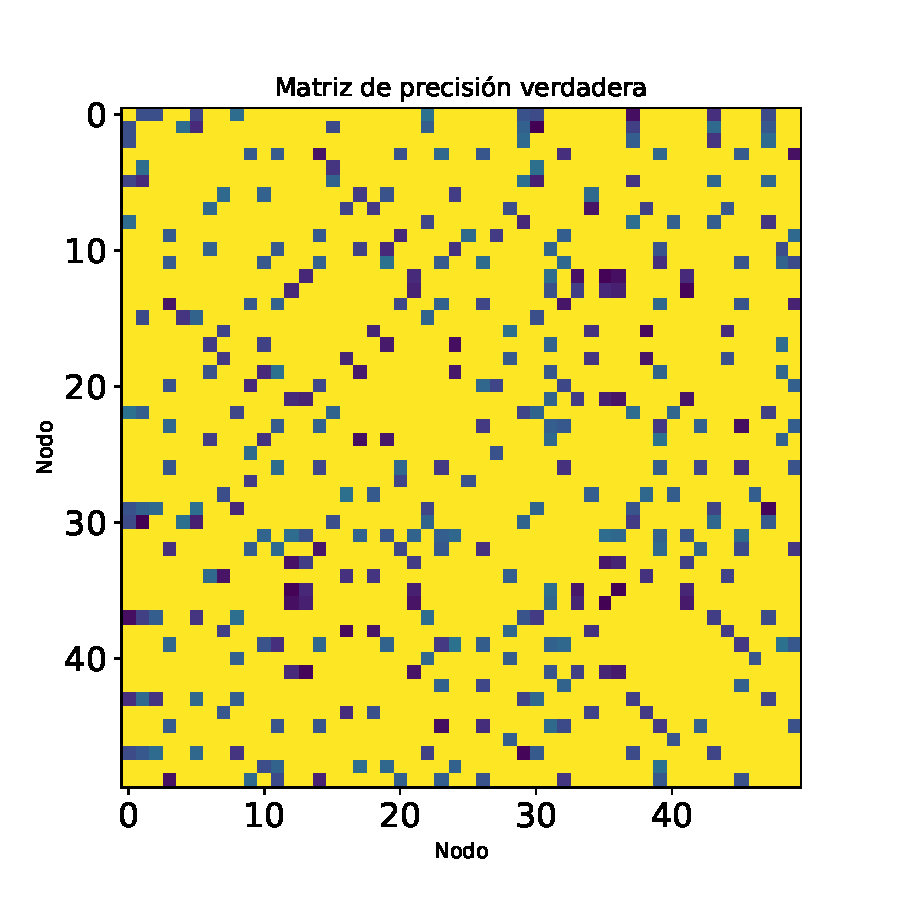
\includegraphics[width=\textwidth]{imagenes/kalofolias/kalofolias_true.pdf}
        \caption*{Matriz verdadera}
    \end{minipage}
    \hfill
    \begin{minipage}[t]{0.72\textwidth}
        \centering
        \begin{tabular}{ccc}
            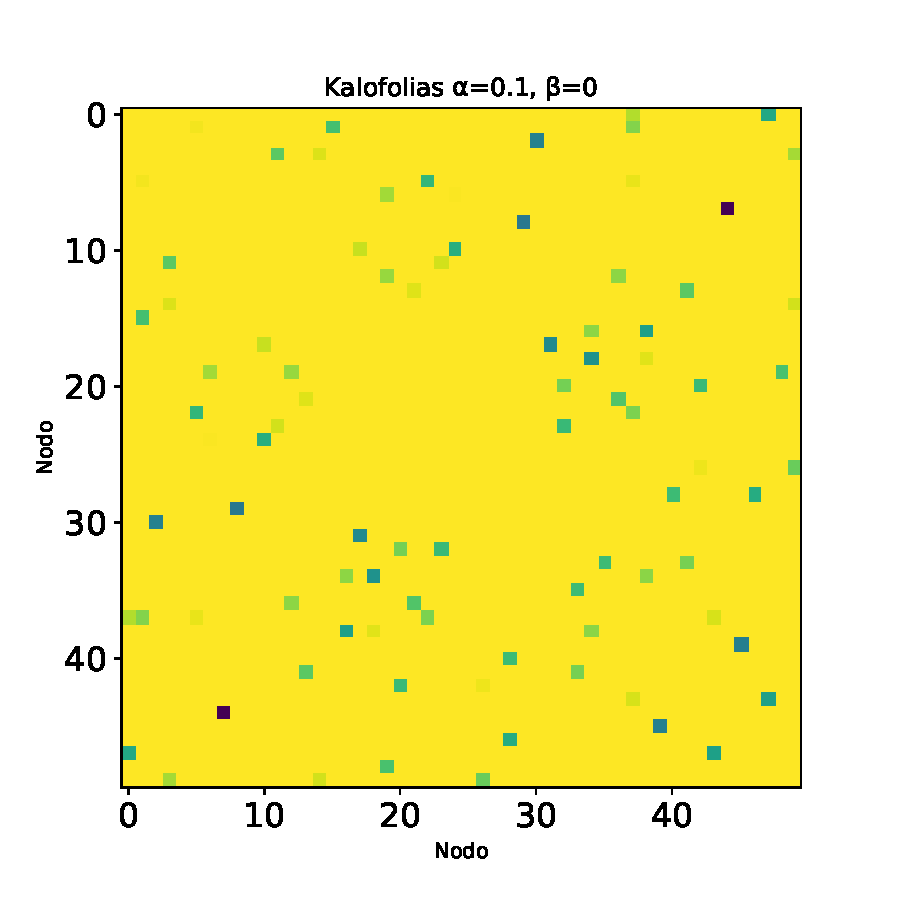
\includegraphics[width=0.28\textwidth]{imagenes/kalofolias/kalofolias_alpha0.1_beta0.pdf} &
            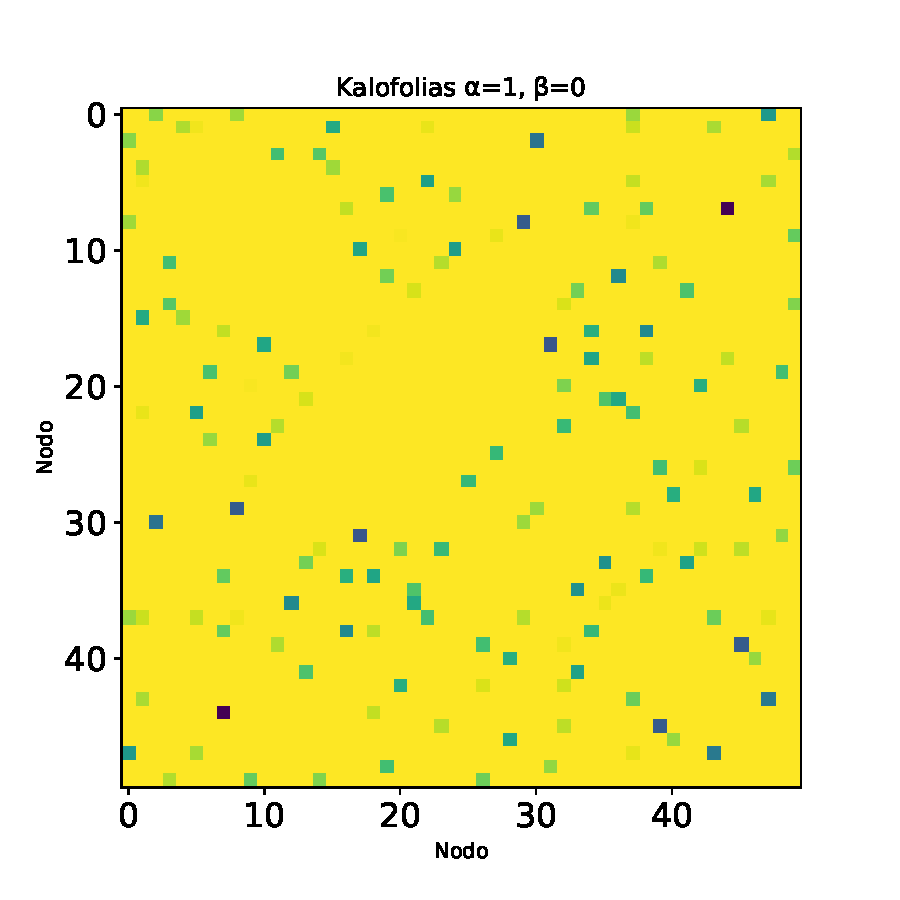
\includegraphics[width=0.28\textwidth]{imagenes/kalofolias/kalofolias_alpha1_beta0.pdf} &
            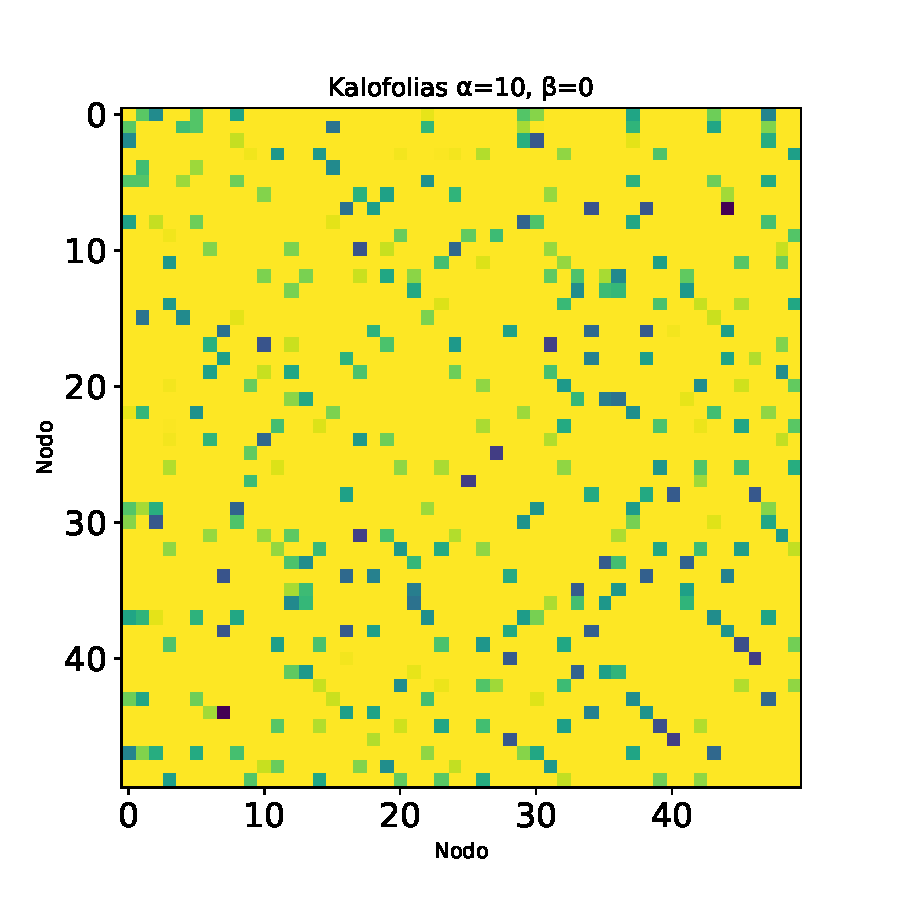
\includegraphics[width=0.28\textwidth]{imagenes/kalofolias/kalofolias_alpha10_beta0.pdf} \\
            $\alpha=0.1$, $\beta=0$ & $\alpha=1$, $\beta=0$ & $\alpha=10$, $\beta=0$ \\[1em]
            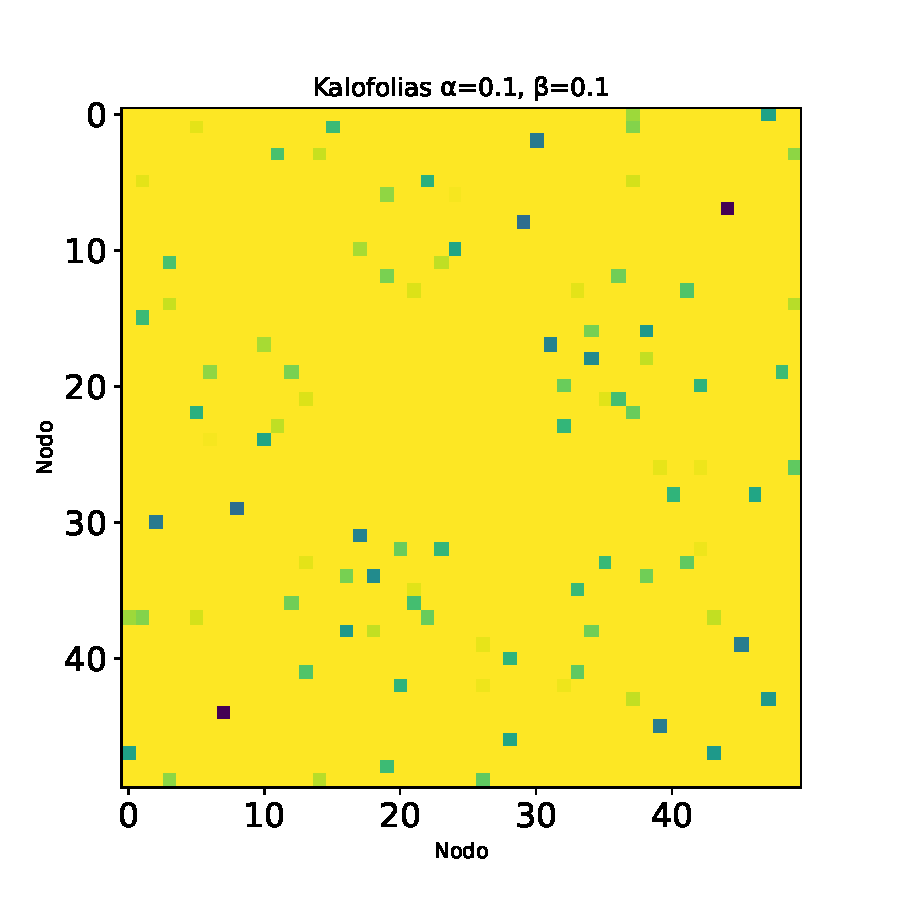
\includegraphics[width=0.28\textwidth]{imagenes/kalofolias/kalofolias_alpha0.1_beta0.1.pdf} &
            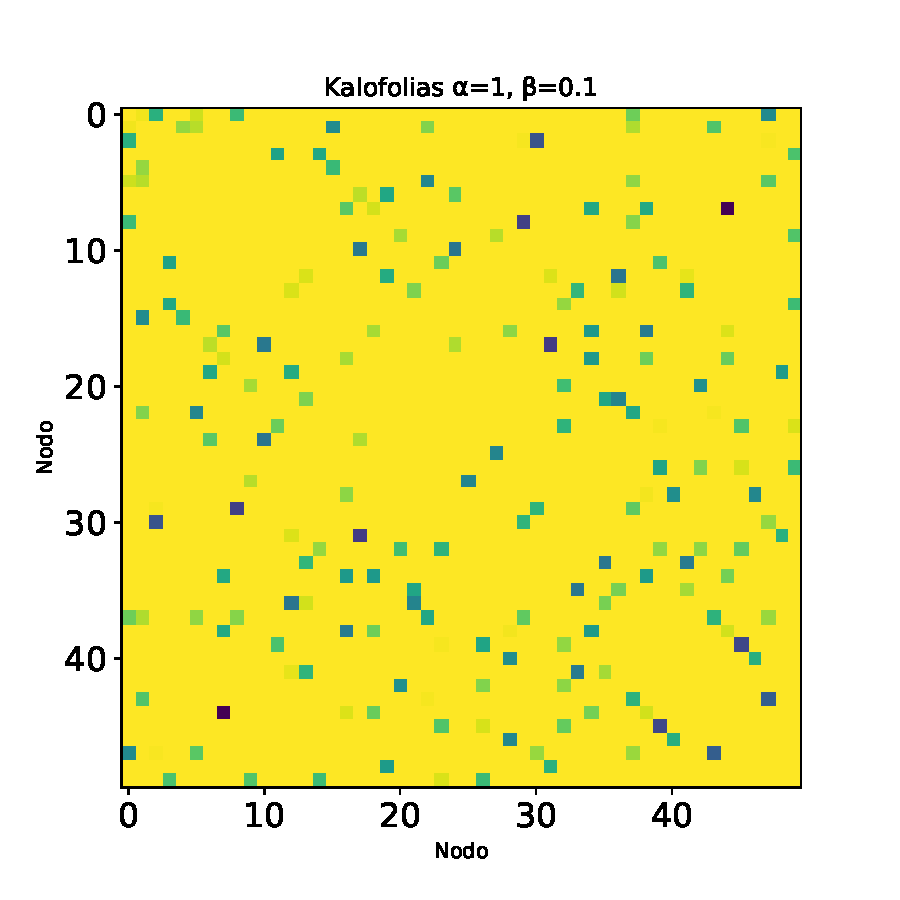
\includegraphics[width=0.28\textwidth]{imagenes/kalofolias/kalofolias_alpha1_beta0.1.pdf} &
            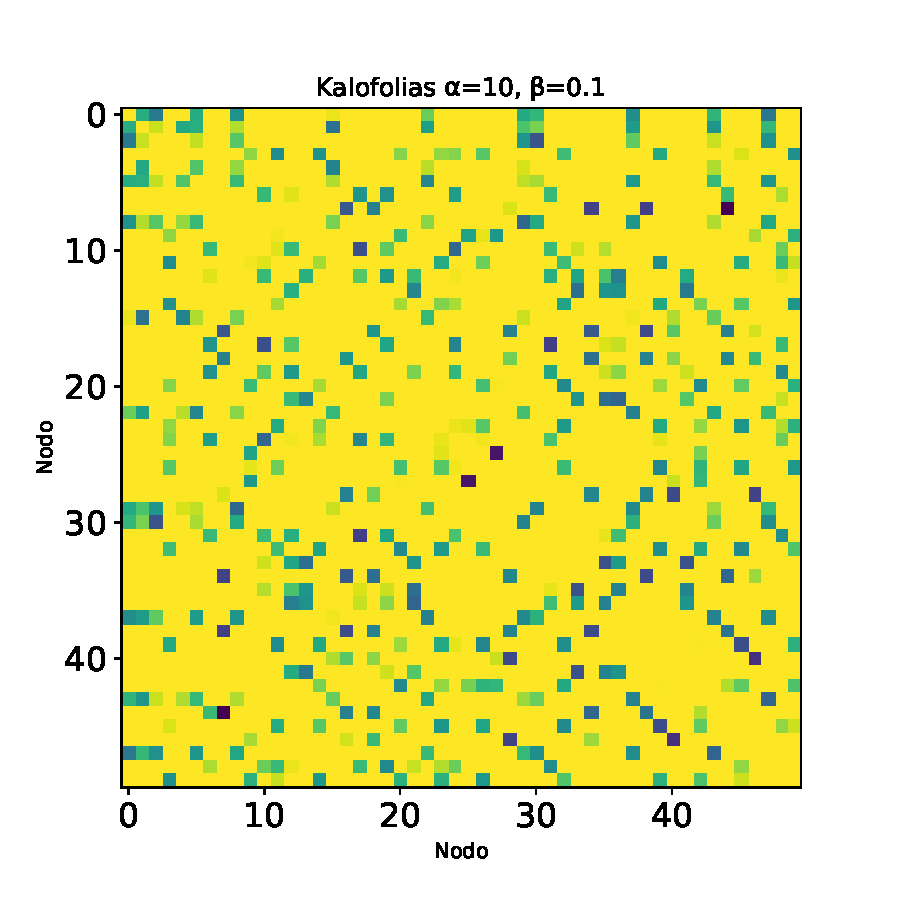
\includegraphics[width=0.28\textwidth]{imagenes/kalofolias/kalofolias_alpha10_beta0.1.pdf} \\
            $\alpha=0.1$, $\beta=0.1$ & $\alpha=1$, $\beta=0.1$ & $\alpha=10$, $\beta=0.1$ \\[1em]
            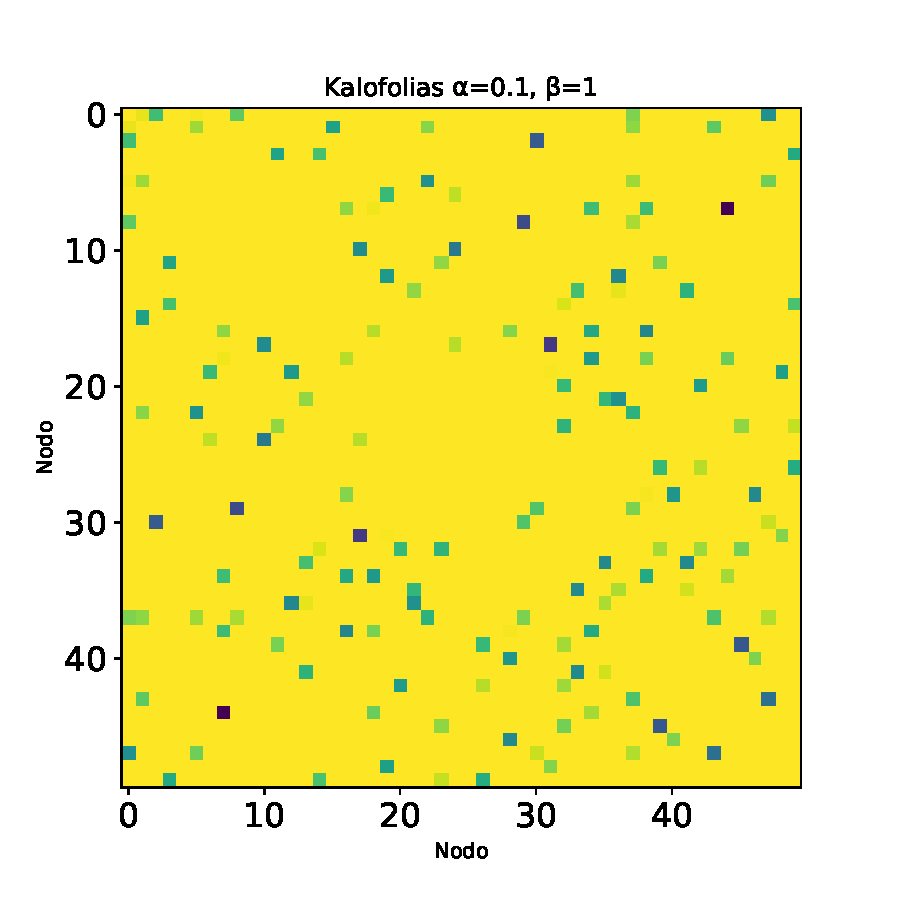
\includegraphics[width=0.28\textwidth]{imagenes/kalofolias/kalofolias_alpha0.1_beta1.pdf} &
            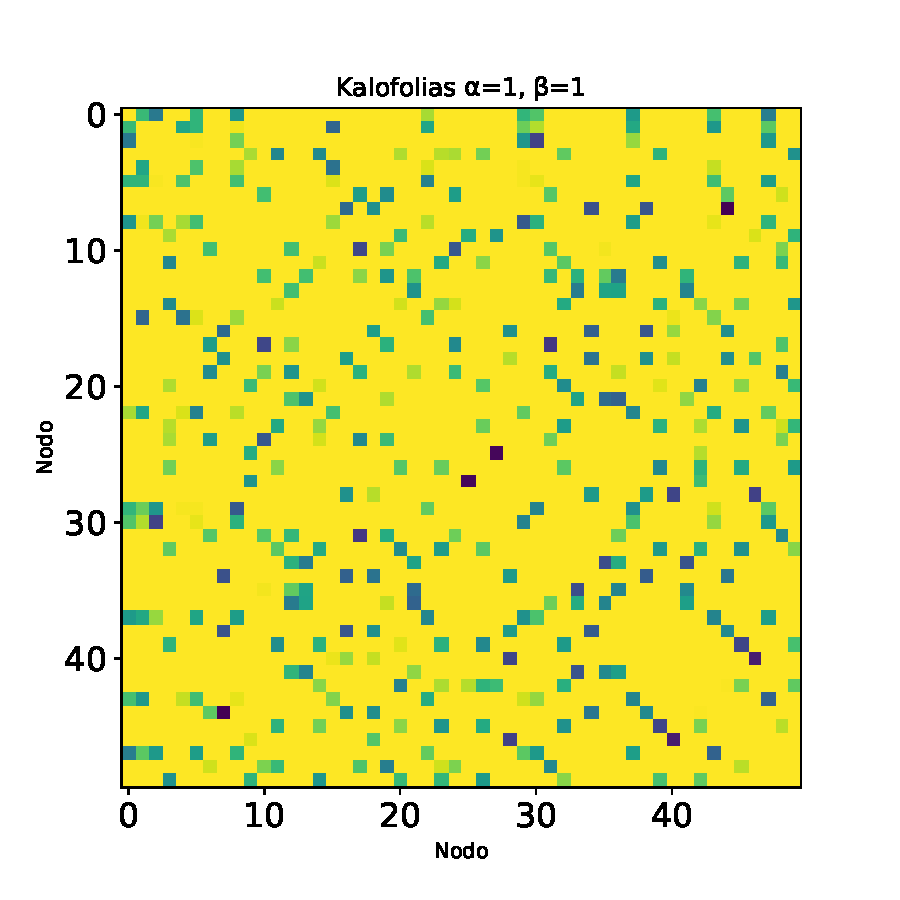
\includegraphics[width=0.28\textwidth]{imagenes/kalofolias/kalofolias_alpha1_beta1.pdf} &
            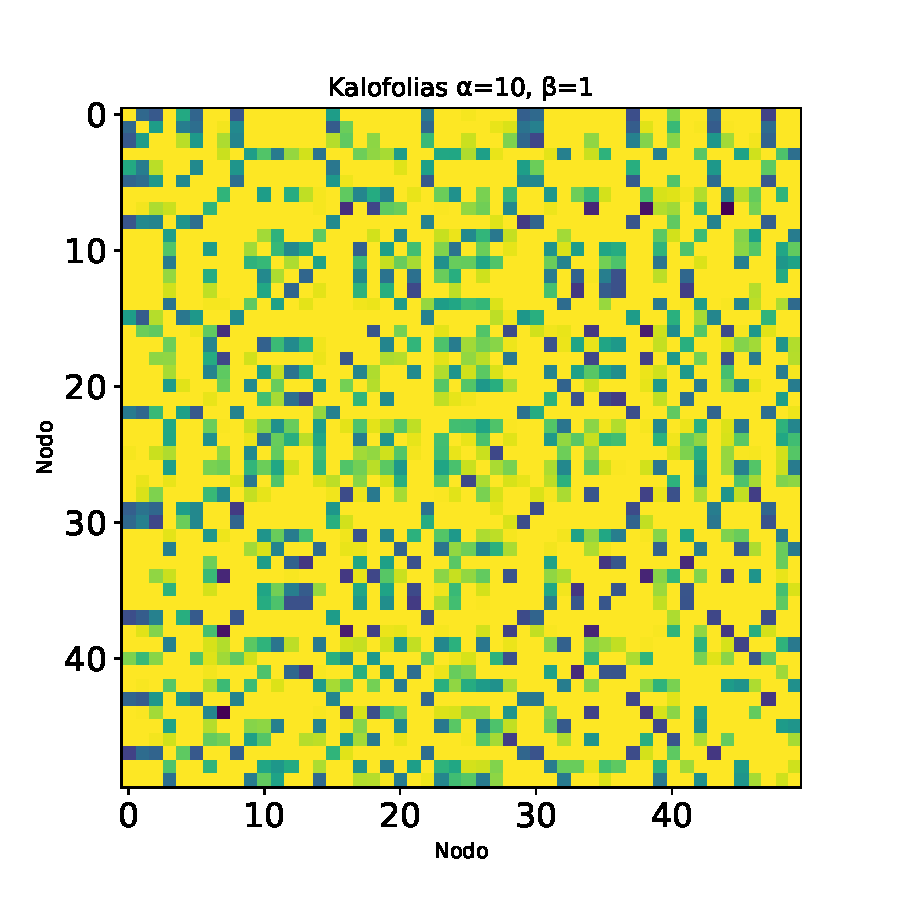
\includegraphics[width=0.28\textwidth]{imagenes/kalofolias/kalofolias_alpha10_beta1.pdf} \\
            $\alpha=0.1$, $\beta=1$ & $\alpha=1$, $\beta=1$ & $\alpha=10$, $\beta=1$ \\
        \end{tabular}
    \end{minipage}
    \caption{Resultados del método de Kalofolias para distintos valores de $\alpha$ y $\beta$, comparados con la matriz verdadera (izquierda) y una grilla 3x3 de variaciones (derecha).}
    \label{fig:kalofolias_grid}
\end{figure}

 

\subsection{Comparación y visualización de los grafos aprendidos}

En la figura \ref{fig:generated_graphs_syntetic} se presenta una comparación visual entre el grafo verdadero y los grafos aprendidos mediante los métodos de Graphical Lasso, Meinshausen y Bühlmann, y Kalofolias. Cada subfigura muestra la estructura de conexiones entre nodos, permitiendo observar las similitudes y diferencias en la topología inferida por cada método en relación con el grafo original.

\begin{figure}[htb]
    \centering
    \begin{subfigure}[t]{0.24\linewidth}
        \centering
        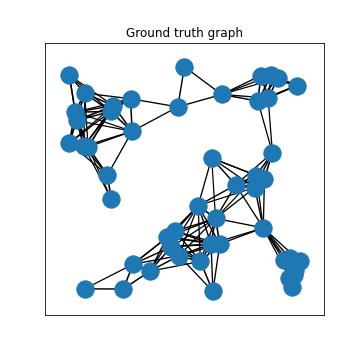
\includegraphics[width=\textwidth]{imagenes/generated_graph_syntetic/ground_truth_graph.png}
        \caption{Grafo verdadero}
    \end{subfigure}\hfill
    \begin{subfigure}[t]{0.24\linewidth}
        \centering
        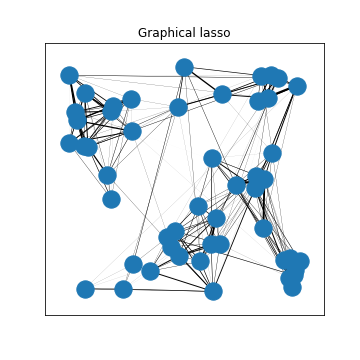
\includegraphics[width=\textwidth]{imagenes/generated_graph_syntetic/graphical_lasso.png}
        \caption{Graphical Lasso}
    \end{subfigure}\hfill
    \begin{subfigure}[t]{0.24\linewidth}
        \centering
        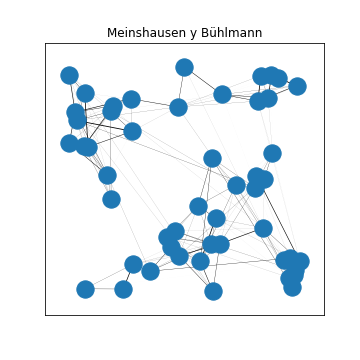
\includegraphics[width=\textwidth]{imagenes/generated_graph_syntetic/meinshausen_buhlmann.png}
        \caption{Meinshausen y Bühlmann}
    \end{subfigure}\hfill
    \begin{subfigure}[t]{0.24\linewidth}
        \centering
        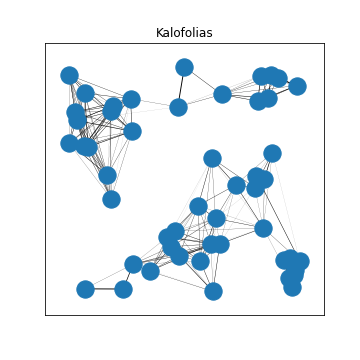
\includegraphics[width=\textwidth]{imagenes/generated_graph_syntetic/kalofolias.png}
        \caption{Kalofolias}
    \end{subfigure}
    \caption{Comparación visual de los grafos: verdadero y aprendidos por distintos métodos.}
    \label{fig:generated_graphs_syntetic}
\end{figure}
La comparación visual de la figura~\ref{fig:generated_graphs_syntetic} muestra que Graphical Lasso recupera bien la estructura principal del grafo, aunque introduce algunas conexiones espurias; Meinshausen y Bühlmann produce un grafo más disperso, capturando solo las conexiones más fuertes y perdiendo muchas débiles; y Kalofolias logra un balance intermedio, con una topología similar pero no idéntica al grafo original. 


\section{Inferencia de topología en MNIST}
Para esta parte trabajaremos el dataset MNIST, que contiene imágenes de dígitos escritos a mano. El objetivo es aprender la estructura del grafo que conecta las imágenes basándonos en sus características visuales, y luego utilizar esta estructura para realizar clustering espectral y evaluar su desempeño.

\subsection{Descripción del dataset y preprocesamiento}
Para trabajar, nos quedaremos con un subconjunto de 2000 imágenes (doscientas por cada dígito) de dimensión $28 \times 28$ píxeles. Cada imagen la convertimos en un vector de dimensión 784 (aplanando la matriz) y normalizamos los valores de píxeles al rango $[0,1]$.

\subsection{Construcción de la matriz de features y t-SNE}

\subsection{Grafo aprendido con Meinshausen y Bühlmann}

\subsection{Grafo aprendido con Kalofolias y umbralización}

\subsection{Clustering espectral sobre grafos aprendidos}

\subsubsection{Métricas de evaluación}

\subsubsection{Resultados y comparación}

\subsection{Visualización en el plano t-SNE por método}

\subsection{Análisis de aciertos y errores por método}


\section{Conclusiones}


\section{Referencias}
\bibliographystyle{plain}
\bibliography{refs}


\end{document}